\chapter{驾驶人行为特性的差异性分析}
\section{数据处理}
\subsection{数据构成}
\subsection{数据筛选}

\section{跟驰行为特性的差异}


\subsection{时间间隔分布}
时间间隔的定义:
取20s以内的时间间隔数据,非专业驾驶人时间间隔分布如图4.1,专业驾驶人时间间隔分布如图4.2。使用对数正态分布进行拟合,0.05显著水平下,卡方检验均不符合对树正态分布,KS检验专业驾驶人符合对数正态分布,非专业驾驶人不符合对数正态分布。专业驾驶人时间间隔整体上小于非专业驾驶人的时间间隔,这符合一般的感性认识。


\subsubsection{非专业}
\begin{figure}[htpb]
	\centering
	\label{tgap_distru:non_pro}
	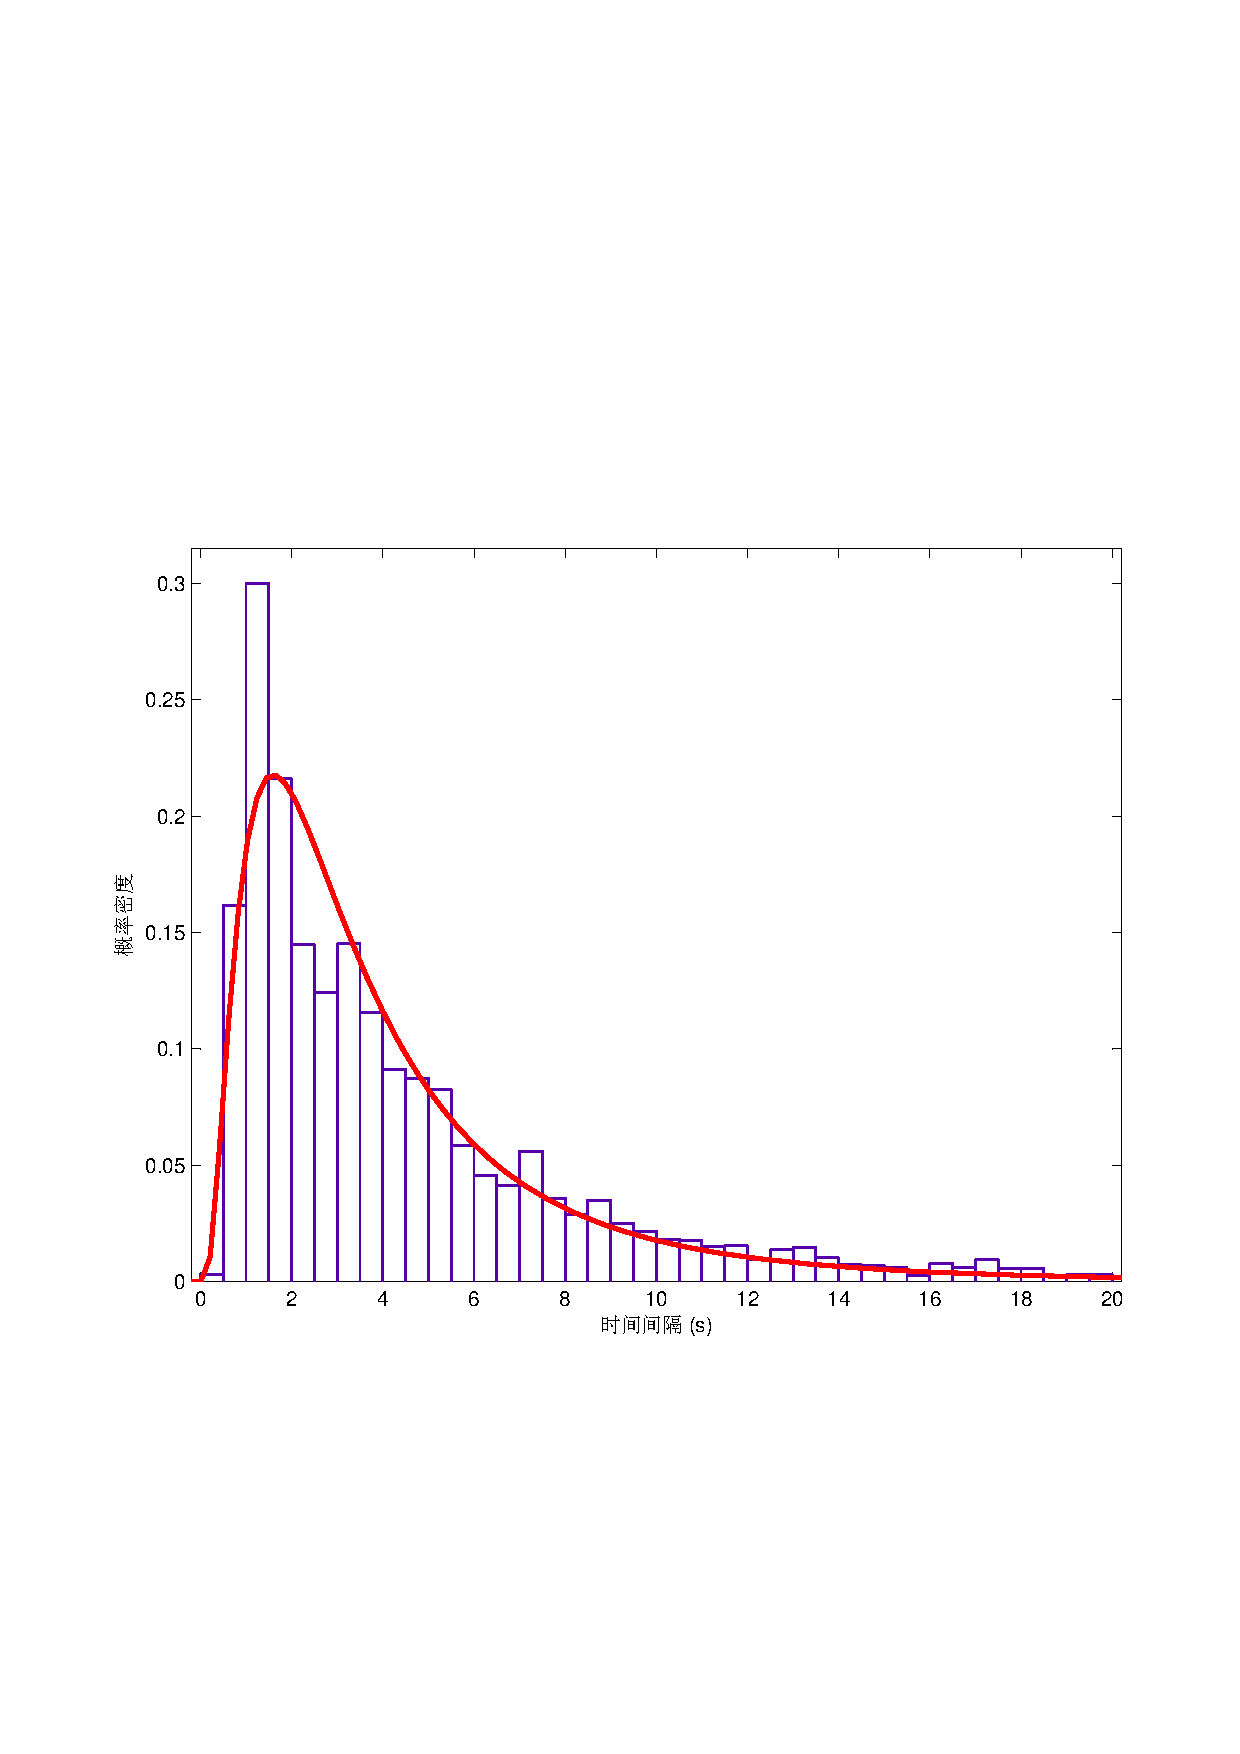
\includegraphics[totalheight=10cm]{o1}
	\caption{非专业驾驶人时间间隔分布}
\end{figure}


Distribution:    Lognormal\\
Log likelihood:  -11056.3\\
Domain:          0 < y < Inf\\
Mean:            4.37392\\
Variance:        18.3609\\

Parameter  Estimate  Std. Err. \\
mu          1.13926   0.0119837\\
sigma      0.820249  0.00847512\\

Estimated covariance of parameter estimates:\\
       mu            sigma       \\
mu      0.000143609  1.51271e-019\\
sigma  1.51271e-019  7.18276e-005\\

检验\\
Chi-square:\\
null hypothesis :服从lognormal分布\\
p= 1.74778427653571e-27<0.05 拒绝\\
KS-test:\\
null hypothesis :服从lognormal分布\\
p= 1.24971275593801e-13<0.05 拒绝\\






\subsubsection{专业}
\begin{figure}[htpb]
	\centering
	\label{tgap_distru:pro}
	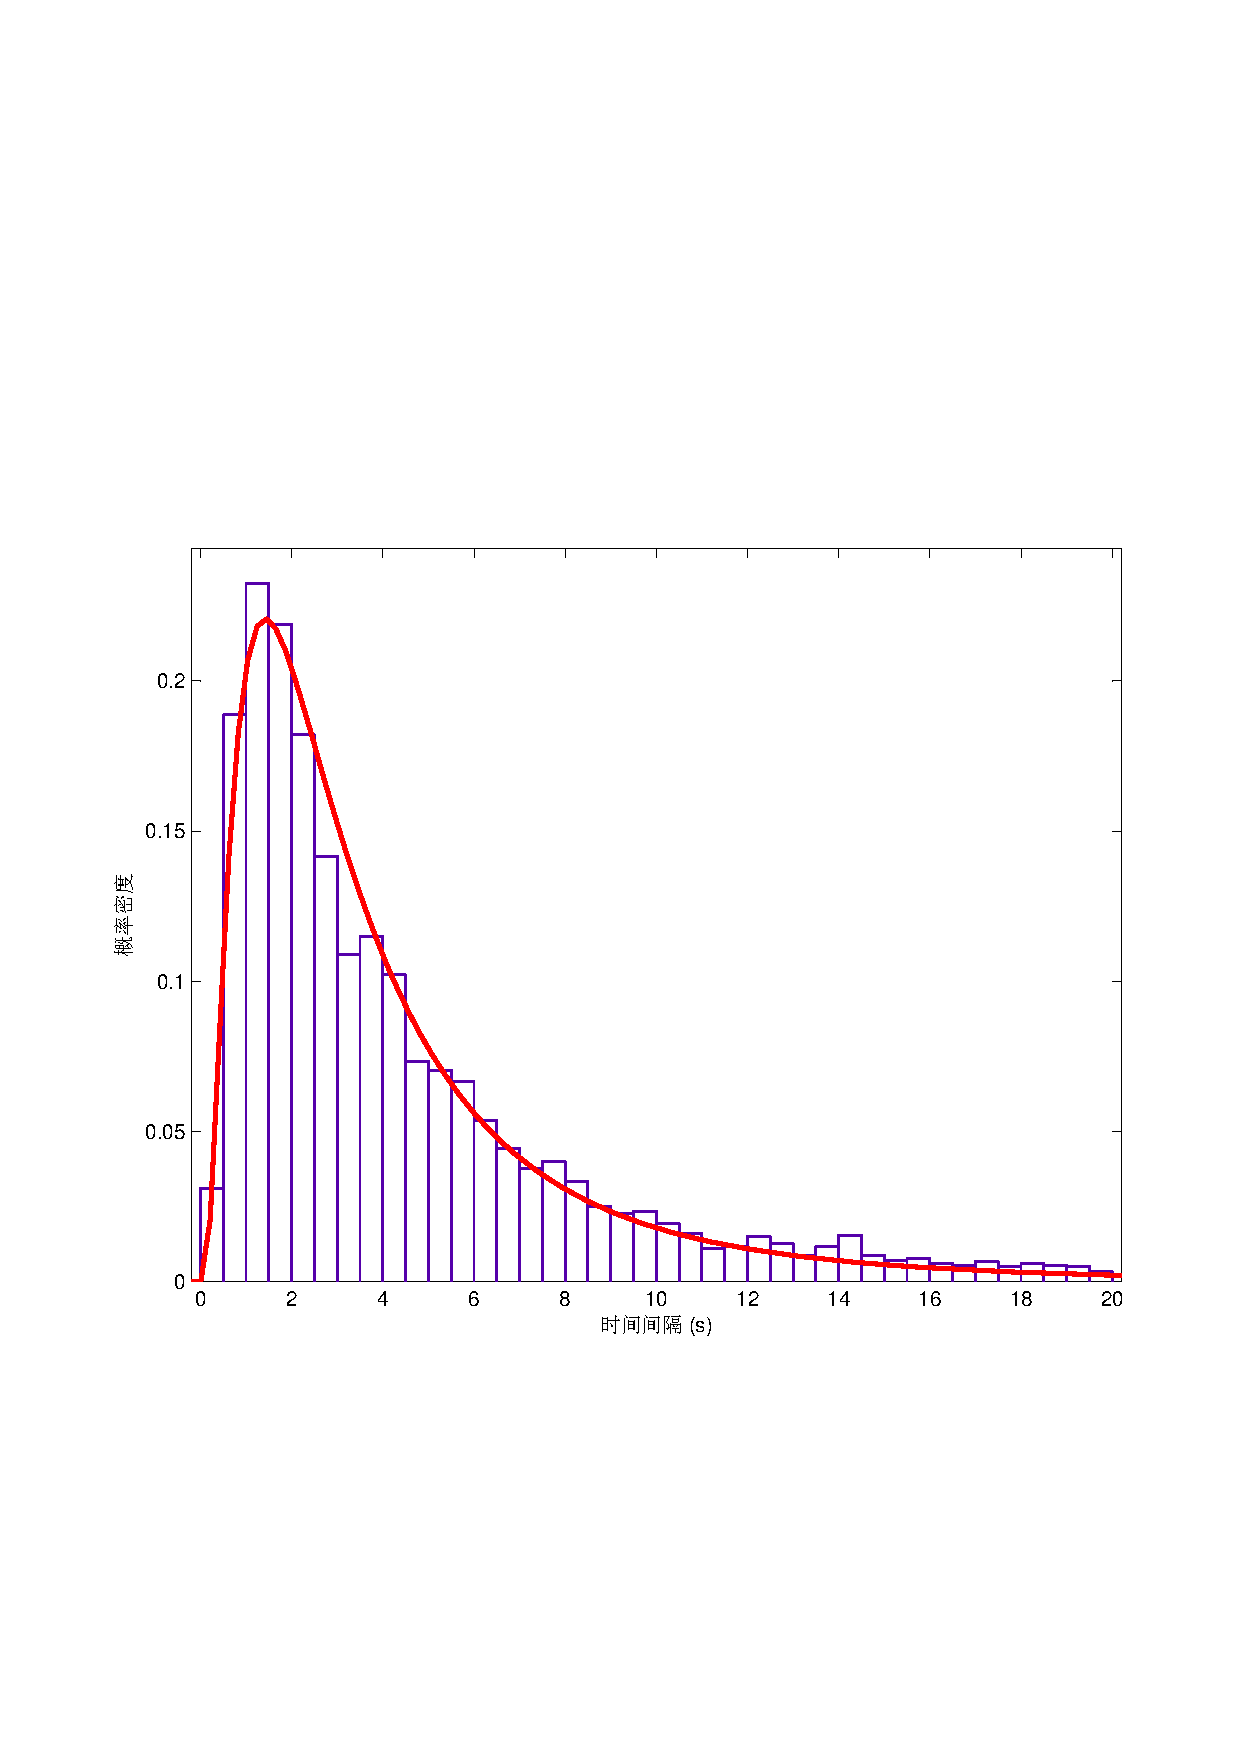
\includegraphics[totalheight=10cm]{o2}
	\caption{专业驾驶人时间间隔分布}
\end{figure}

Distribution:    Lognormal\\
Log likelihood:  -8615.43\\
Domain:          0 < y < Inf\\
Mean:            4.43296\\
Variance:        22.3341\\

Parameter  Estimate  Std. Err.\\
mu          1.10947  0.0145138\\
sigma      0.871312  0.0102649\\

Estimated covariance of parameter estimates:\\
       mu             sigma        \\
mu        0.00021065  -2.79065e-019\\
sigma  -2.79065e-019    0.000105369\\


检验\\
Chi-square:\\
null hypothesis :服从lognormal分布\\
p= 2.17243543058168e-13<0.05 拒绝\\

KS-test:\\
null hypothesis :服从lognormal分布\\
p= 0.0575478261225268>0.05 接受\\

\subsection{速度--跟驰距离}
对于每一个驾驶人根据速度划分区间对跟车速度和跟驰距离进行平均,得到平均意义上的跟车速度和跟驰距离,从图4.3和图4.4可以看出,无论是非专业还是专业驾驶人,在图形下方均有一条较为明显的趋势线呈现相对线性的关系,同时均存在较大的变化,表明跟驰行为中存在驾驶人其跟车速度和跟驰距离较为偏离线性关系这一假设。从图中看专业驾驶人的变化情况似乎大于专业驾驶人,可以推测专业驾驶人存在更多的不同驾驶类型。
\begin{figure}[htpb]
	\centering
	\label{spd_dist:nonpro}
	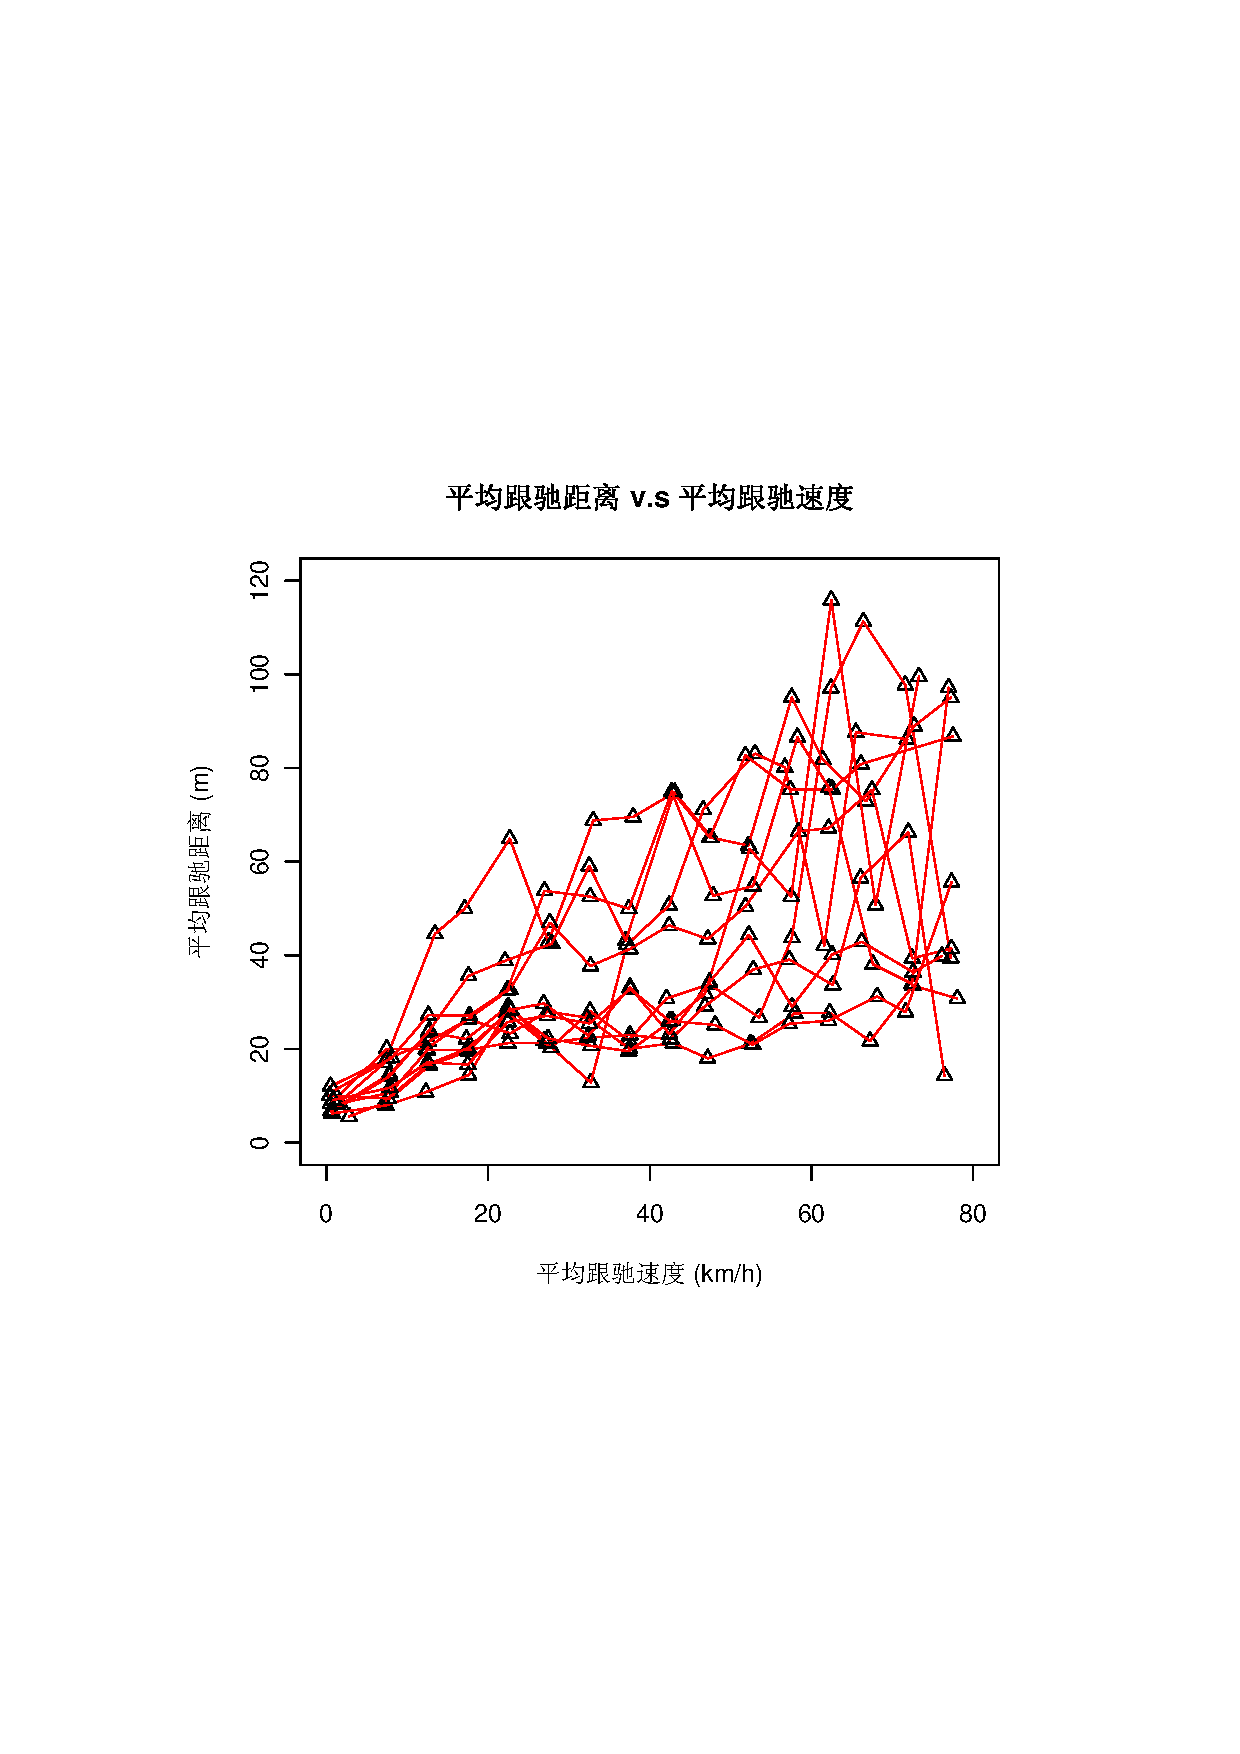
\includegraphics[totalheight=10cm]{non_spd_dist}
	\caption{非专业驾驶人速度--跟驰距离}
\end{figure}



\begin{figure}[htpb]
	\centering
	\label{spd_dist:pro}
	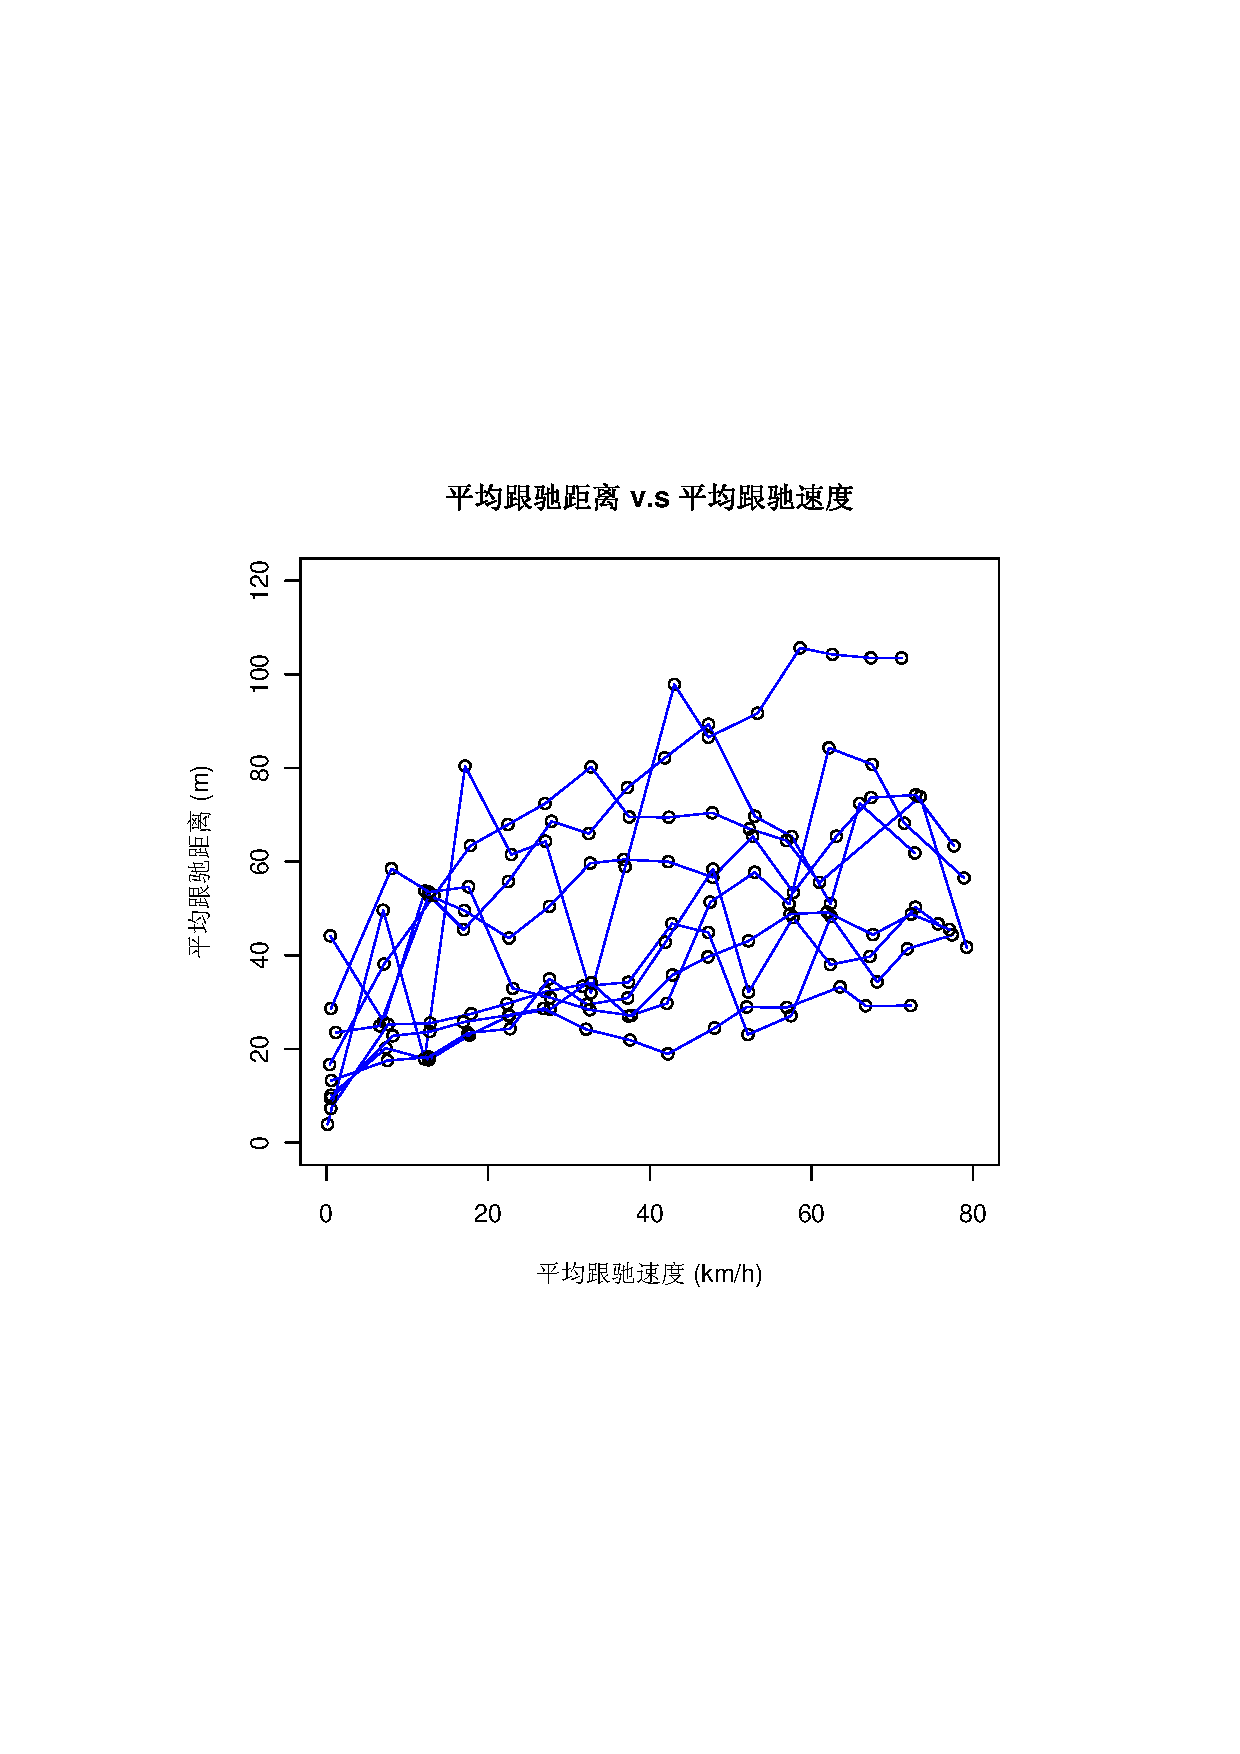
\includegraphics[totalheight=10cm]{pro_spd_dist}
	\caption{专业驾驶人速度--跟驰距离}
\end{figure}

\begin{figure}[htpb]
	\centering
	\label{spd_dist:all}
	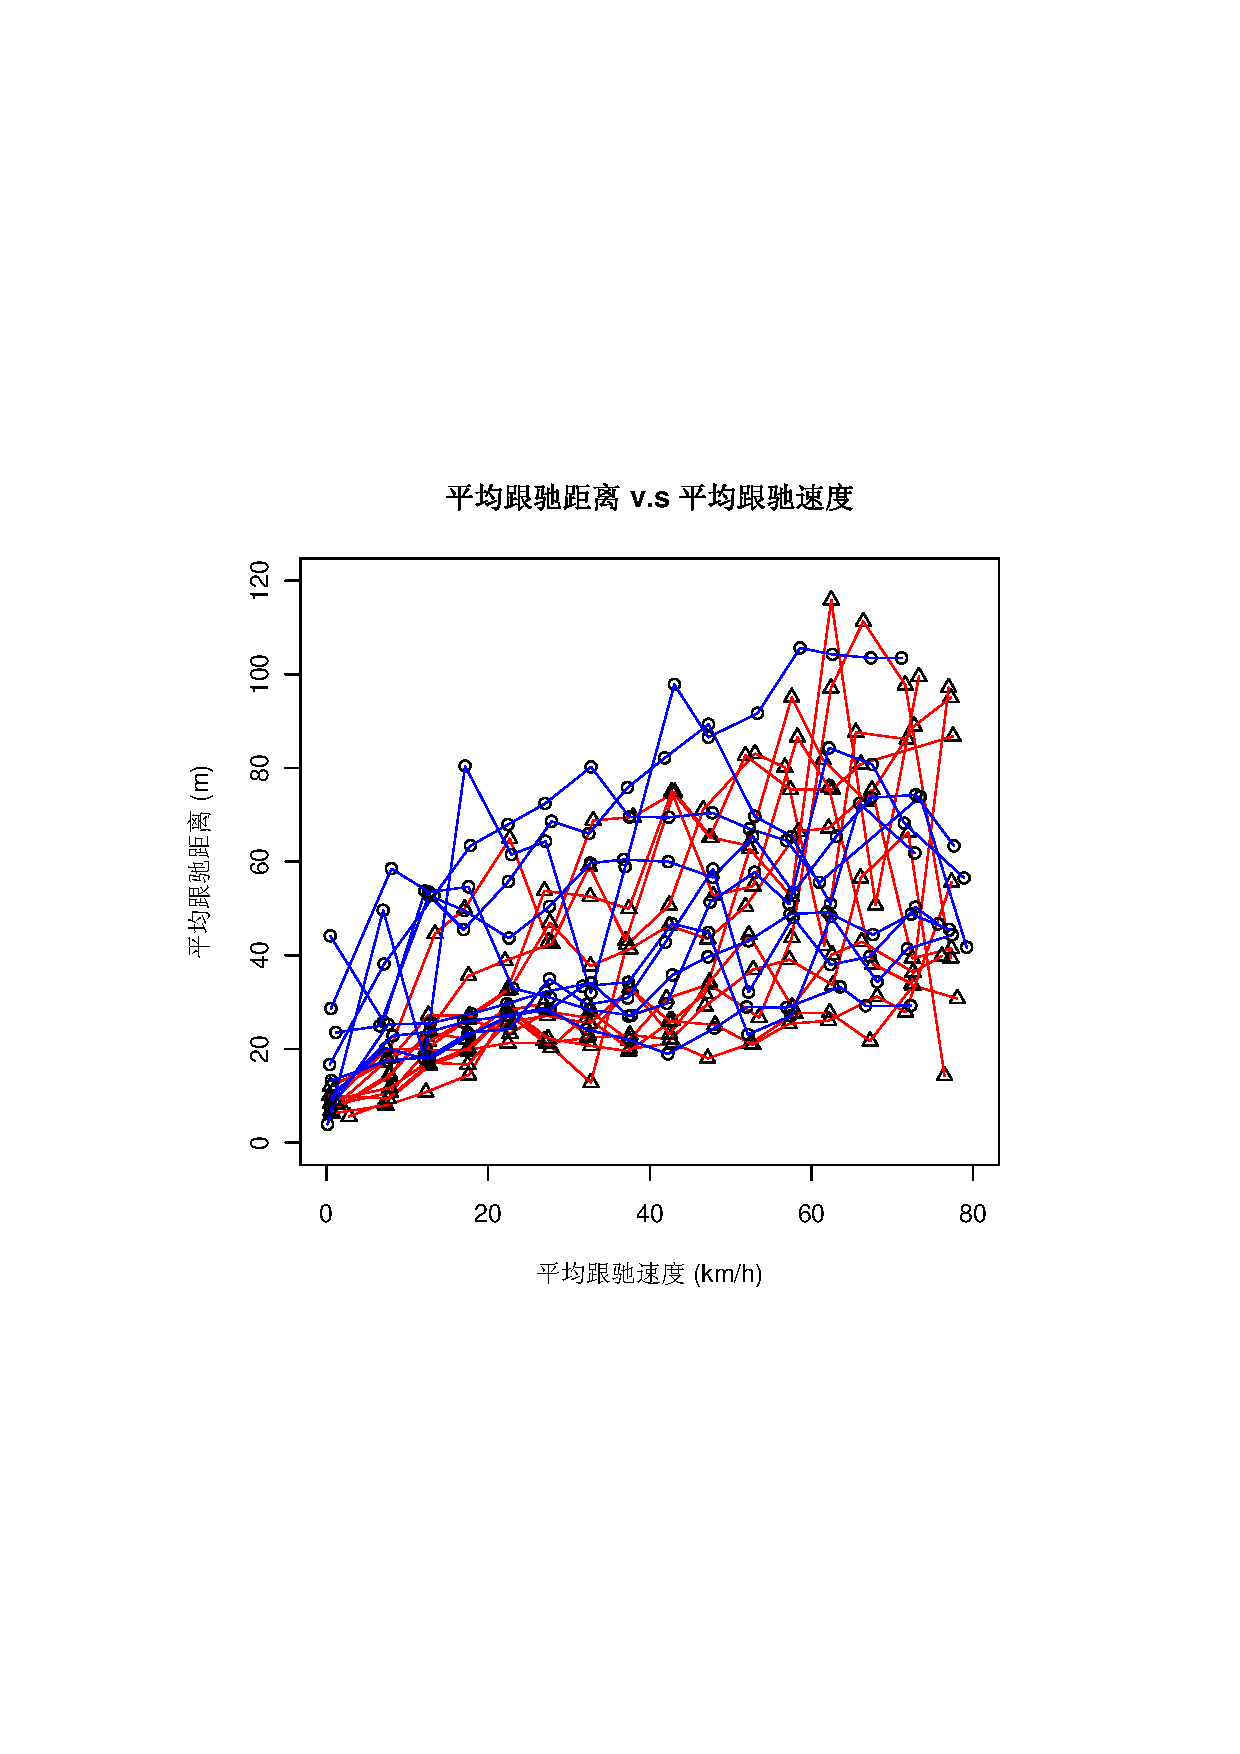
\includegraphics[totalheight=10cm]{all_spd_dist}
	\caption{专业、非专业驾驶人速度--跟驰距离比较}
\end{figure}



\subsection{加速度--相对速度}

对于每一个驾驶人根据相对速度划分区间对加速度和相对速度进行平均,得到平均意义上的加速度和相对速度,从图4.6和图4.7可以看出,无论是非专业还是专业驾驶人,从整体趋势上呈现左低右高,意味着本车速度大于前车速度时有减速的趋势,反之亦反。而图中没有呈现明显的线性变化,而是呈现较大的随机性,跟驰模型中一般假设驾驶人加速度与速度差紧密相关,虽然其具有良好的数学特性,但是实际情况中驾驶人具有非即时反应性,有计划性,这一假设相比于速度与跟驰距离的假设而言是较为严格的假设。同时从图中可以看出代表不同驾驶人的折线变化较大,这表明驾驶人的驾驶类型存在较大差异。
\begin{figure}[htpb]
	\centering
	\label{rspd_acc:nonpro}
	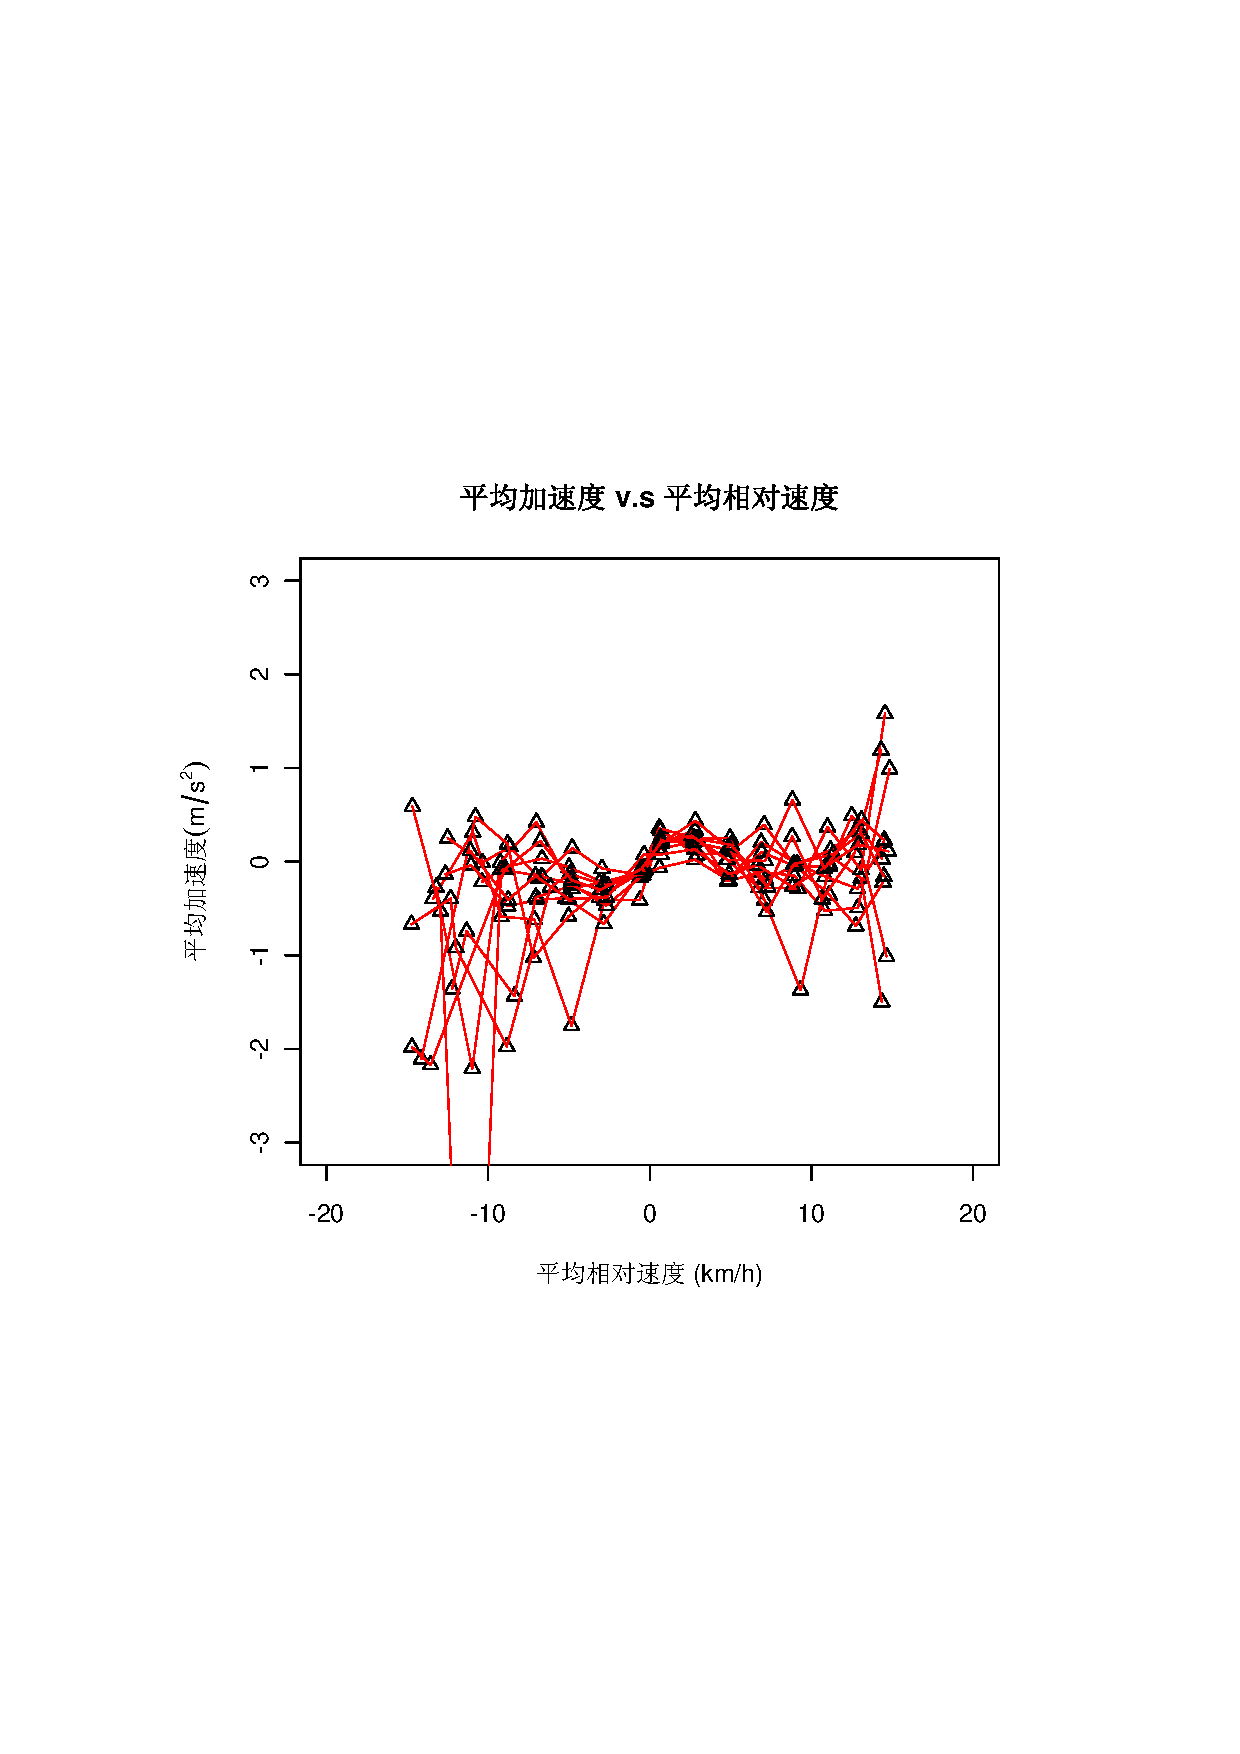
\includegraphics[totalheight=10cm]{non_rspd_acc}
	\caption{非专业驾驶人加速度--相对速度}
\end{figure}

\begin{figure}[htpb]
	\centering
	\label{rspd_acc:pro}
	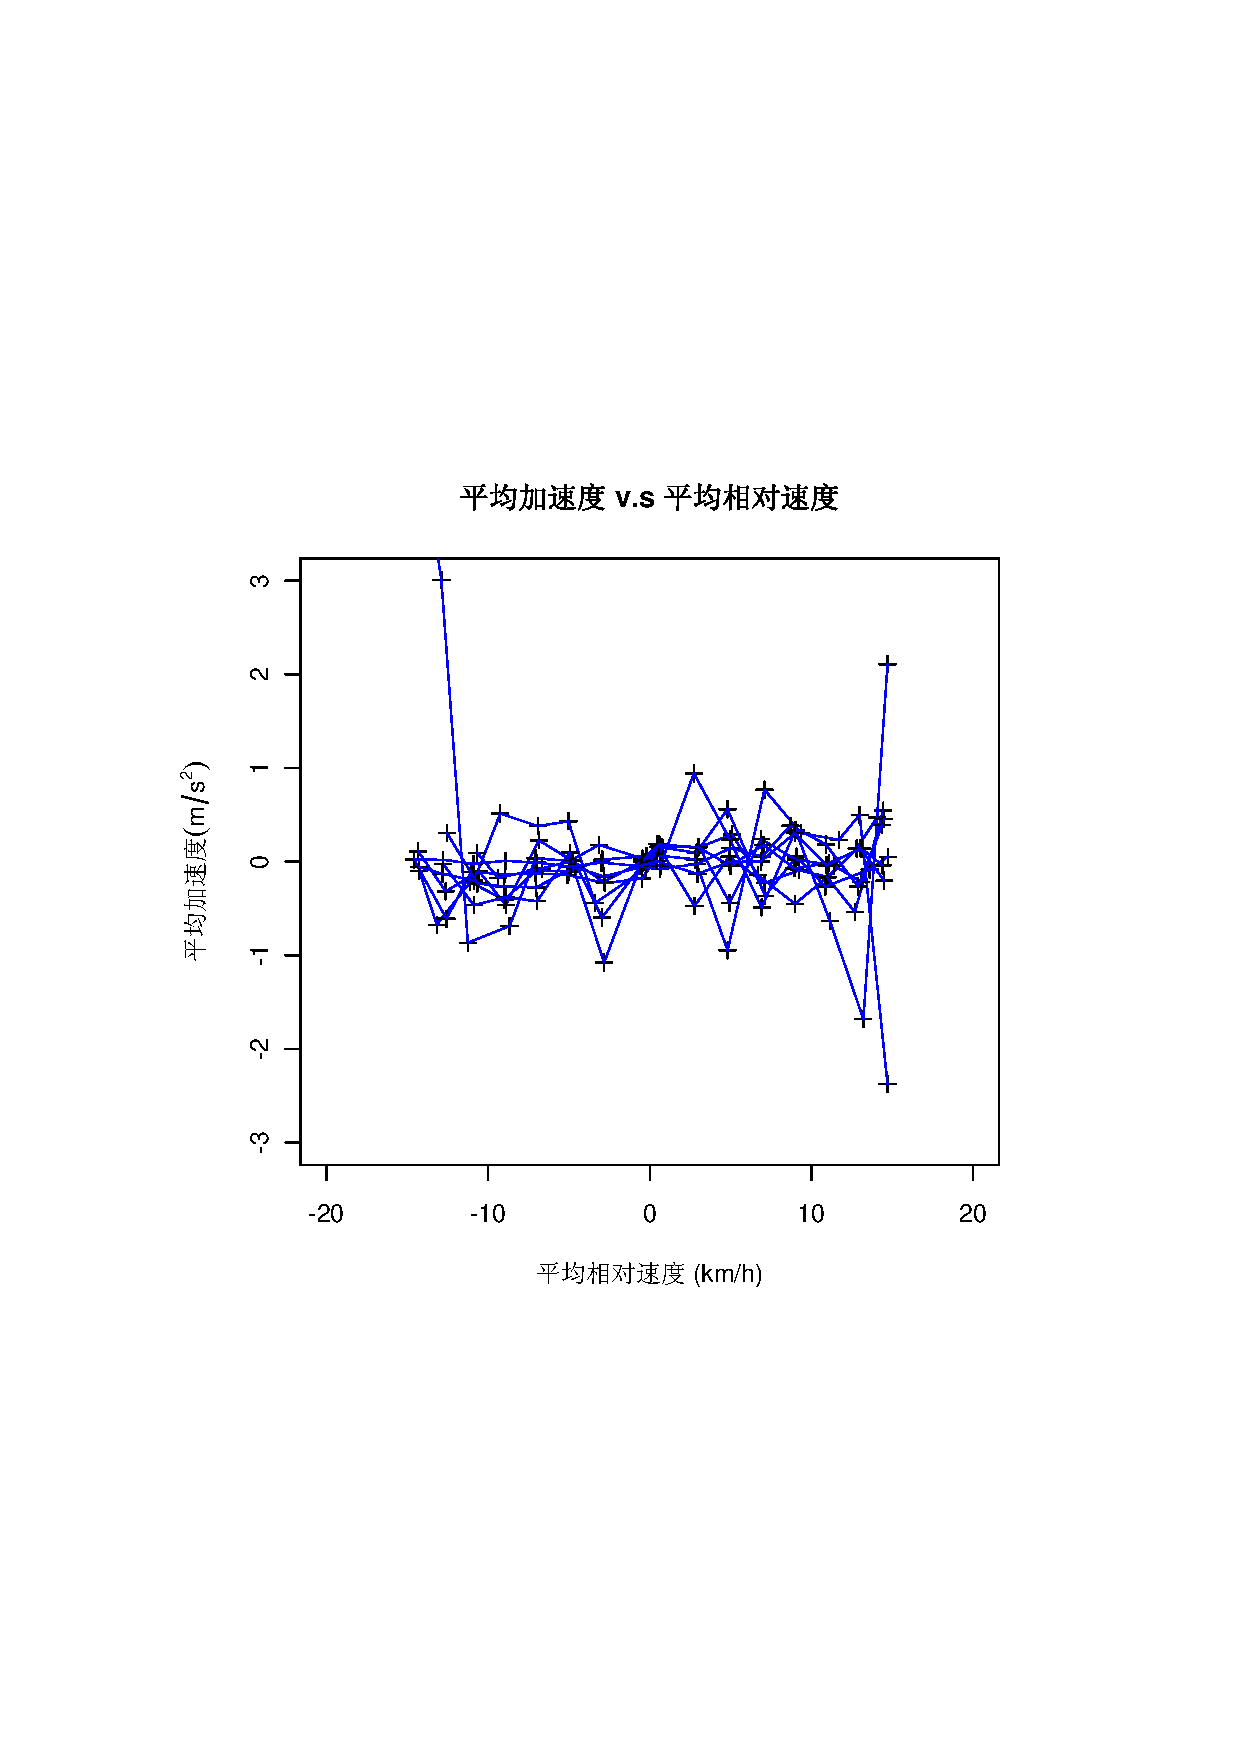
\includegraphics[totalheight=10cm]{pro_rspd_acc}
	\caption{专业驾驶人加速度--相对速度}
\end{figure}

\begin{figure}[htpb]
	\centering
	\label{rspd_acc:all}
	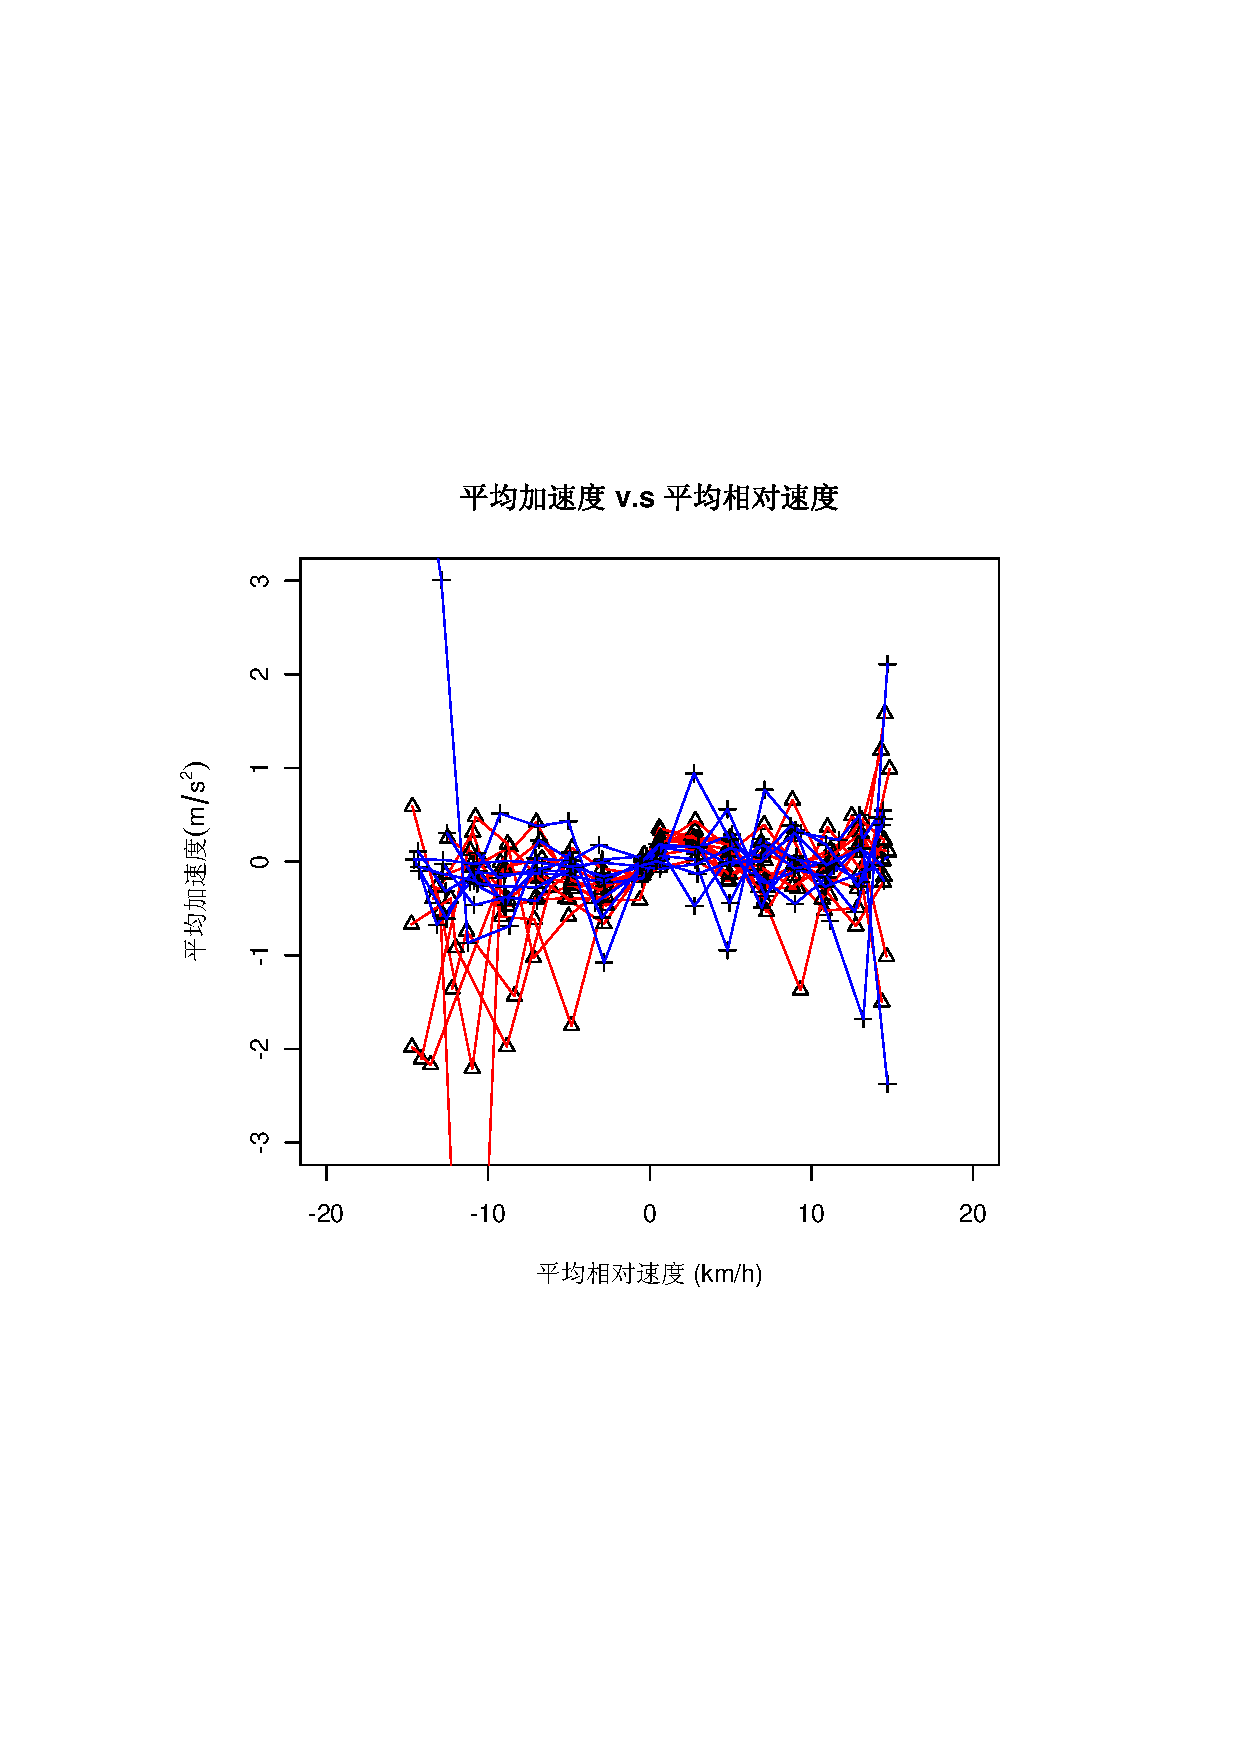
\includegraphics[totalheight=10cm]{all_rspd_acc}
	\caption{专业、非专业驾驶人加速度--相对速度比较}
\end{figure}

%\subsection{速度、加速度特性差异}
%
%\subsection{跟驰距离特性差异}
%\subsection{时间间隔特性差异}
%\begin{figure}[htpb]
%\includegraphics[totalheight=10cm]{Graph1}
%\end{figure}
\subsection{对不同跟驰模型的参数标定及其表现比较}
不同的跟驰模型的不同假设,可以体现驾驶人的不同驾驶类型。通过每条跟驰轨迹使用不同跟驰模型的参数标定,并进行模型拟合程度表现的比较,可以定量化的研究驾驶人的驾驶类型差异。

本文中将选取
\subsubsection{各模型简述}
\subsubsection{轨迹数据的平滑处理}
\subsubsection{参数标定方法}
\subsubsection{模型拟合程度的量化}
\subsubsection{比较结果}




\section{变道选择与间隙接受特性差异}

\section{驾驶人行为特性相关性分析}